\section{Simbologia. Divisão de circuitos}

\begin{frame}{Simbologia}
	\begin{block}{}
		A fim de facilitar a \textbf{execução do projeto} e a \textbf{identificação} dos diversos \textbf{pontos de utilização}, utilizamos \textbf{símbolos gráficos}.

		\medskip

		Os símbolos gráficos utilizados nos projetos de instalações elétricas são \textbf{padronizados} pela ABNT, através das seguintes normas:
		\begin{itemize}
			\item NBR 5444: símbolos gráficos para instalações prediais;
			\item NBR 5446: símbolos gráficos de relacionamento usados na confecção de esquemas;
			\item NBR 5453: sinais e símbolos para eletricidade.
		\end{itemize}
	\end{block}
\end{frame}


\begin{frame}{Simbologia}
	\begin{block}{}
		\begin{itemize}
			\item Na tabela a seguir temos os símbolos gráficos para os projetos de instalações elétricas.
			\item Foram deixadas uma coluna para a simbologia mais usual e uma coluna para a simbologia normalizada pela ABNT, ficando \textbf{a critério de cada projetista }a simbologia a adotar.
		\end{itemize}
	\end{block}

	%	\centering
	%	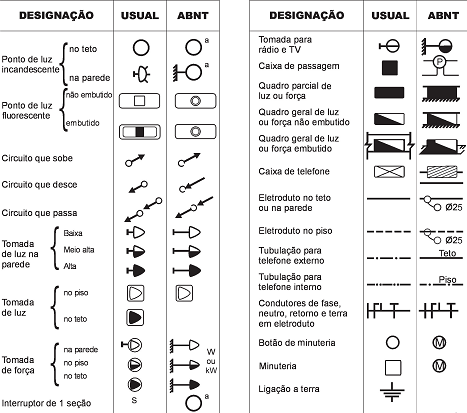
\includegraphics[width=0.7\linewidth]{Figuras/Ch05/fig1}

\end{frame}


\begin{frame}{Simbologia}
	\centering
	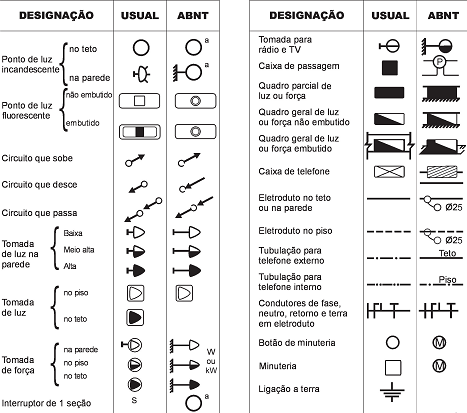
\includegraphics[width=0.74\linewidth]{Figuras/Ch05/fig1}
\end{frame}


\begin{frame}{Simbologia}
	\centering
	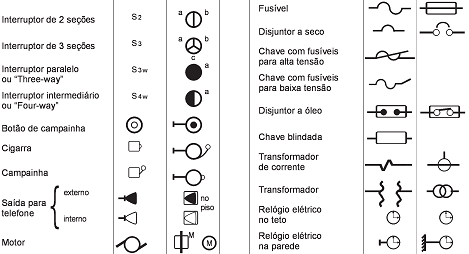
\includegraphics[width=1\linewidth]{Figuras/Ch05/fig2}
\end{frame}


\begin{frame}{Simbologia - Exemplo \#01}
	\centering
	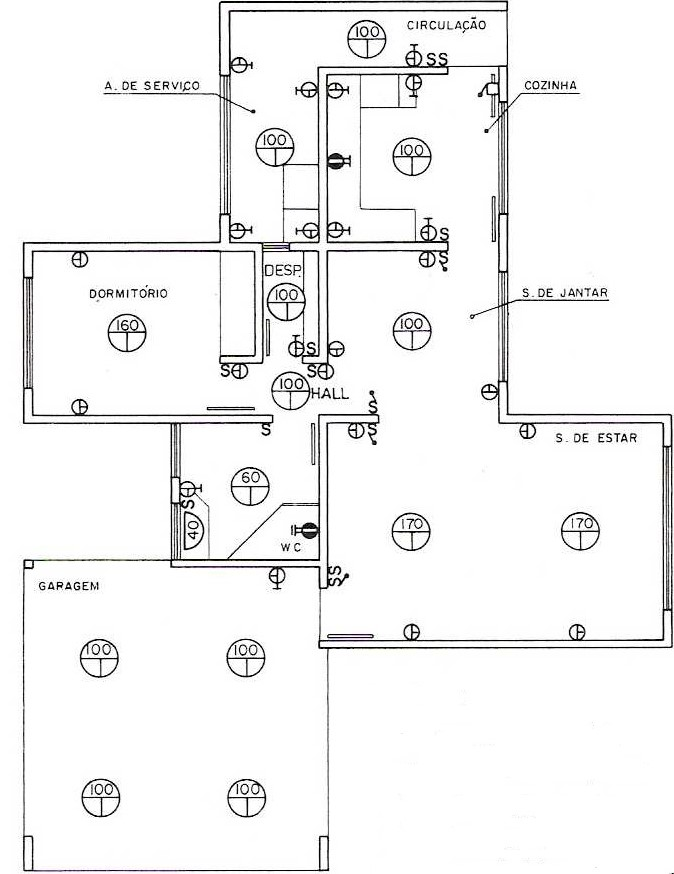
\includegraphics[width=0.5\linewidth]{Figuras/Ch05/fig3}
\end{frame}


\begin{frame}{Simbologia - Exemplo \#01}
	\centering
	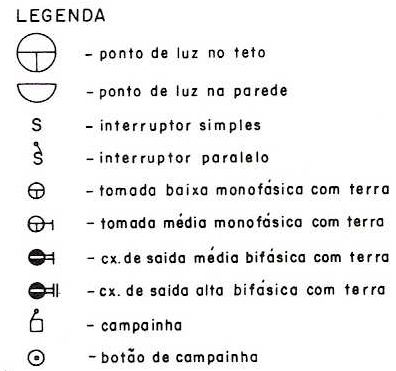
\includegraphics[width=0.7\linewidth]{Figuras/Ch05/fig4}
\end{frame}


\begin{frame}{Divisão da instalação em circuitos - Setores}
	\begin{block}{Quadro de Distribuição (QD) ou Quadro de Luz (QL)}
		\begin{itemize}
			\item Trata-se do componente de uma instalação elétrica destinado a abrigar um ou mais \textbf{dispositivos de proteção} e/ou de \textbf{manobra} e a \textbf{conexão de condutores elétricos} interligados aos mesmos, com o fim de \textbf{distribuir} a energia elétrica aos diversos circuitos.
			\item Recebe os condutores (Ramal de Alimentação) que vêm do medidor ou centro de medição.
		\end{itemize}
		%Fig. 2.9. Quadro de distribuição
	\end{block}

	%	\centering
	%	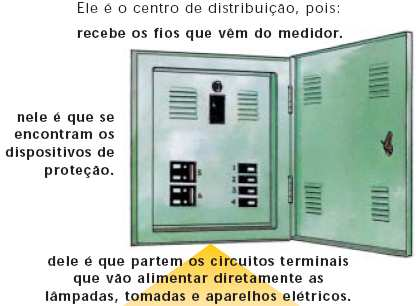
\includegraphics[width=0.4\linewidth]{Figuras/Ch05/fig5}
\end{frame}


\begin{frame}{Divisão da instalação em circuitos - Setores}
	\centering
	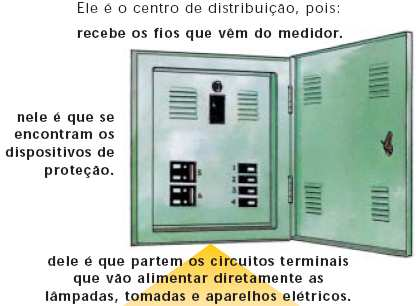
\includegraphics[width=0.8\linewidth]{Figuras/Ch05/fig5}
\end{frame}


\begin{frame}{Divisão da instalação em circuitos}
	\begin{block}{}
		As \textbf{partes componentes} de um \textbf{quadro de distribuição} são:
		\begin{itemize}
			\item Disjuntor Geral;
			\item Barramento de Interligação das Fases;
			\item Disjuntores dos Circuitos Terminais;
			\item Barramento de Neutro;
			\item Barramento de Proteção;
			\item Estrutura: Composta de caixa metálica, chapa de montagem dos componentes, isoladores, tampa e sobretampa.
		\end{itemize}

		A figura a seguir ilustra um exemplo de um quadro de distribuição para fornecimento bifásico.


		%Fig. 2.10 Exemplo de quadro de distribuição para fornecimento bifásico.
	\end{block}

	%	\centering
	%	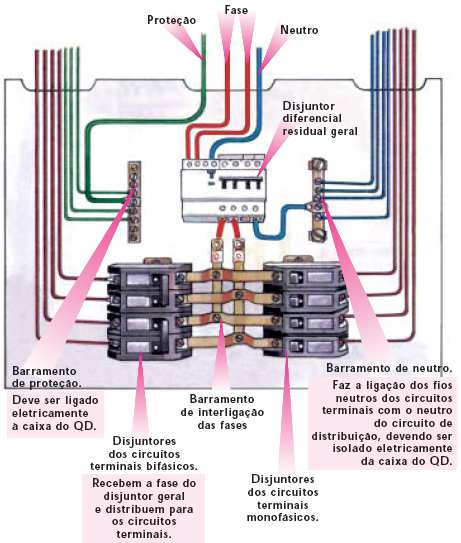
\includegraphics[width=0.7\linewidth]{Figuras/Ch05/fig6}
\end{frame}

\begin{frame}{Divisão da instalação em circuitos}
	\centering
	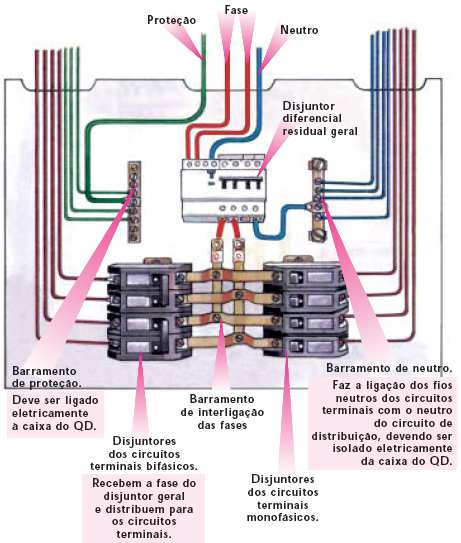
\includegraphics[width=0.55\linewidth]{Figuras/Ch05/fig6}
\end{frame}


\begin{frame}{Divisão da instalação em circuitos}
	\begin{block}{Circuito Elétrico}
		\begin{itemize}
			\item É o conjunto de \textbf{equipamentos} e \textbf{fios} ligados ao mesmo \textbf{dispositivo de proteção}.
			\item Em uma instalação elétrica residencial, encontramos dois tipos de circuito:
			      \begin{itemize}
				      \item\normalsize o de \textbf{distribuição}, e;
				      \item\normalsize os \textbf{circuitos terminais}.
			      \end{itemize}
		\end{itemize}
	\end{block}
\end{frame}


\begin{frame}{Divisão da instalação em circuitos - Circuito Elétrico}
	\centering
	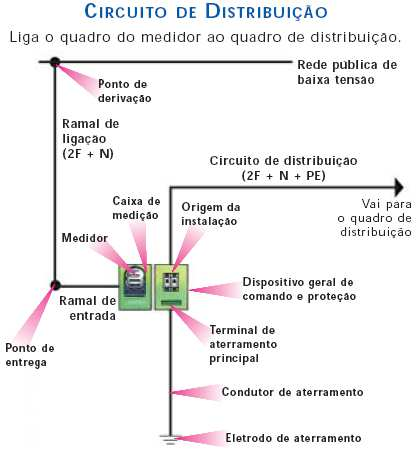
\includegraphics[width=0.6\linewidth]{Figuras/Ch05/fig7}
\end{frame}


\begin{frame}{Divisão da instalação em circuitos}
	\begin{block}{}
		A figura abaixo ilustra um exemplo de circuitos terminais protegidos por disjuntores	termomagnéticos.
	\end{block}

	\centering
	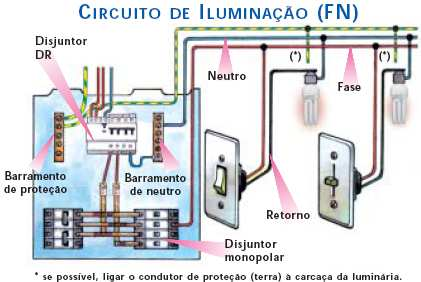
\includegraphics[width=0.7\linewidth]{Figuras/Ch05/fig8}
\end{frame}


\begin{frame}{Divisão da instalação em circuitos}
	\begin{block}{}
		Exemplo de circuitos terminais protegidos por disjuntores DR:
	\end{block}

	\bigskip

	\begin{minipage}{0.49\linewidth}
		\centering
		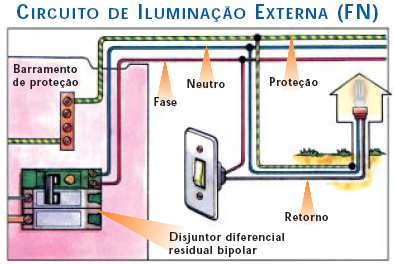
\includegraphics[width=1\linewidth]{Figuras/Ch05/fig9}
	\end{minipage}\hfill
	\begin{minipage}{0.49\linewidth}
		\centering
		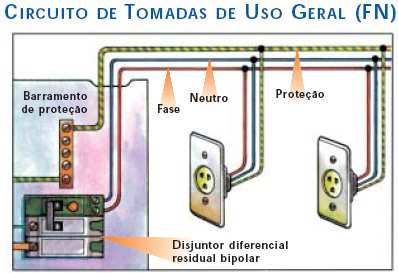
\includegraphics[width=1\linewidth]{Figuras/Ch05/fig10}
	\end{minipage}
\end{frame}


\begin{frame}{Divisão da instalação em circuitos}
	\begin{minipage}{0.49\linewidth}
		\centering
		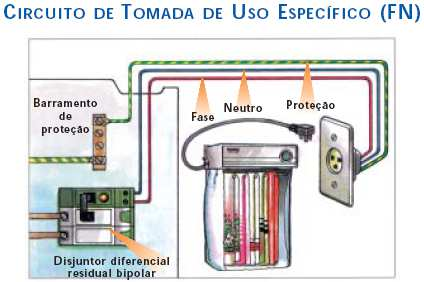
\includegraphics[width=1\linewidth]{Figuras/Ch05/fig11}
	\end{minipage}\hfill
	\begin{minipage}{0.49\linewidth}
		\centering
		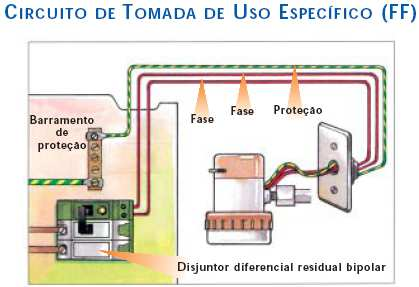
\includegraphics[width=1\linewidth]{Figuras/Ch05/fig12}
	\end{minipage}
\end{frame}


\begin{frame}{Divisão da instalação em circuitos}
	\begin{minipage}{0.49\linewidth}
		\centering
		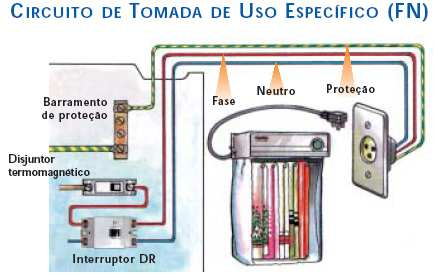
\includegraphics[width=1\linewidth]{Figuras/Ch05/fig13}
	\end{minipage}\hfill
	\begin{minipage}{0.49\linewidth}
		\centering
		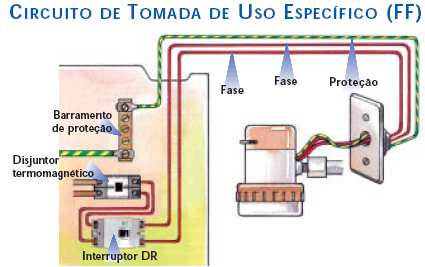
\includegraphics[width=1\linewidth]{Figuras/Ch05/fig14}
	\end{minipage}
\end{frame}


\begin{frame}{Divisão da instalação em circuitos}
	\begin{block}{Quadros Terminais}
		\begin{itemize}
			\item São quadros elétricos que alimentam \textbf{exclusivamente} circuitos terminais.
		\end{itemize}
	\end{block}

	\begin{block}{Circuitos Alimentadores}
		\begin{itemize}
			\item São os circuitos que alimentam \textbf{um ou mais} quadros terminais e/ou quadros de distribuição (alimentadores).
			\item Os termos: circuitos de distribuição principal, circuito de distribuição divisionário e circuito subalimentador são também empregados para designar circuitos alimentadores.
			\item Os circuitos alimentadores podem ser \textbf{monofásicos}, \textbf{bifásicos }ou \textbf{trifásicos}.
			\item Os circuitos alimentadores partem de uma \textbf{fonte de energia} (rede pública, transformador ou gerador) ou de um \textbf{quadro de distribuição }e alimentam um ou mais quadros.
		\end{itemize}
	\end{block}
\end{frame}


\begin{frame}{Divisão da instalação em circuitos}
	\begin{block}{Quadros Alimentadores ou Quadros de Distribuição}
		\begin{itemize}
			\item São os quadros dos quais partem um ou mais circuitos alimentadores, podendo também partir, dos mesmos, circuitos terminais.
		\end{itemize}
	\end{block}

	\centering
	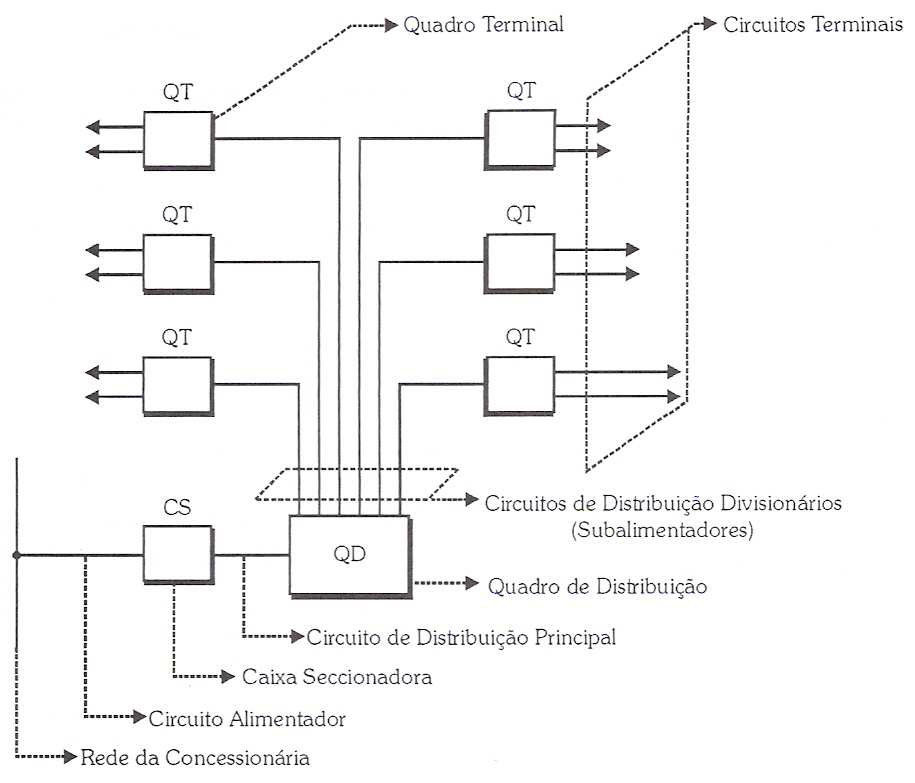
\includegraphics[width=0.55\linewidth]{Figuras/Ch05/fig15}
\end{frame}


\begin{frame}{Divisão da instalação em circuitos terminais}
	\begin{block}{Introdução}
		\begin{itemize}
			\item É de fundamental importância que toda instalação elétrica seja \textbf{dividida}, de acordo com as necessidades, \textbf{em vários circuitos}, devendo \textbf{cada circuito} ser concebido de forma a \textbf{poder ser seccionado sem risco de realimentação inadvertida} através de outros circuitos.
			\item Também é importante ter em mente que os circuitos devem ter \textbf{pouca carga}, para que sua utilização seja mais prática.
			\item Se os circuitos ficarem muito carregados, os fios adequados para suas ligações irão resultar numa \textbf{seção nominal} (bitola) \textbf{muito grande} (acima de \SI{4.0}{\milli\meter\squared}), dificultando:

			      \begin{itemize}
				      \item\normalsize a \textbf{instalação dos fios} nos eletrodutos;
				      \item\normalsize as \textbf{ligações terminais} (interruptores e tomadas).
			      \end{itemize}
		\end{itemize}
	\end{block}
\end{frame}


\begin{frame}{Divisão da instalação em circuitos terminais}
	\begin{block}{}
		\begin{itemize}
			\item A divisão em circuitos terminais facilitará a \textbf{operação} e \textbf{manutenção} da instalação, além de \textbf{reduzir a interferência entre os pontos de utilização}.
			\item Como consequência, os \textbf{circuitos terminais individualizados }terão reduzidas a \textbf{queda de tensão }e a corrente nominal, o que possibilitará o \textbf{dimensionamento }de \textbf{condutores }e \textbf{dispositivos de proteção }de \textbf{menor seção }e \textbf{capacidade nominal}.
			\item Cada \textbf{circuito terminal }será ligado a um \textbf{dispositivo de proteção}. No caso das instalações residências, poderão ser utilizados \textbf{disjuntores termomagnéticos }ou \textbf{disjuntores residuais diferenciais }(DR).
		\end{itemize}

	\end{block}
\end{frame}


\begin{frame}{Divisão da instalação em circuitos terminais}
	\begin{block}{Circuitos normais}
		Em instalações de \textbf{alto padrão técnico }devem haver \textbf{circuitos normais }e \textbf{circuitos de segurança}.
		\begin{itemize}
			\item Os circuitos \textbf{normais }estão ligados \textbf{apenas a uma fonte}, em geral, \textbf{à concessionária local}.
			      Em caso de \textbf{falha da rede}, haverá \textbf{interrupção no abastecimento}.
			\item Estes circuitos são muitas vezes chamados de \textit{não-essenciais}.
		\end{itemize}
	\end{block}
	\vspace{-0.1cm}
	\begin{block}{Circuitos de segurança}
		\begin{itemize}
			\item Os \textbf{circuitos de segurança }são aqueles que \textbf{garantirão o abastecimento}, mesmo quando houver falha da concessionária.
			\item Como exemplo podem-se citar os \textbf{circuitos de alarme }e de \textbf{proteção contra incêndio}, abastecidos \textbf{simultaneamente }pela \textbf{concessionária }e por \textbf{fonte própria }(baterias, geradores de emergência etc.).
			\item Os circuitos de segurança são muitas vezes chamados de \textit{essenciais}.
		\end{itemize}
	\end{block}
\end{frame}


\begin{frame}{Divisão da instalação em circuitos terminais}
	\begin{block}{Objetivos}
		A divisão da instalação em circuitos terminais tem os seguintes objetivos:
		\begin{itemize}
			\item Limitar as consequências de uma falha, a qual provocará apenas o seccionamento do circuito defeituoso;
			\item Facilitar as verificações, os ensaios e a manutenção;
			\item Evitar os perigos que possam resultar da falha de um circuito único, como no caso de iluminação.
		\end{itemize}
	\end{block}
\end{frame}


\begin{frame}{Divisão da instalação em circuitos terminais}
	\begin{block}{Critérios para a divisão da instalação em circuitos terminais}
		\begin{itemize}
			\item Os circuitos terminais devem ser \textbf{individualizados} pela \textbf{função} dos equipamentos de utilização que alimentam. Em particular, devem ser previstos circuitos terminais \textbf{distintos} para \textbf{iluminação} e \textbf{tomadas}.
			\item Em unidades \textbf{residenciais}, \textbf{hotéis}, \textbf{motéis }ou \textbf{similares }são permitidos pontos de \textbf{iluminação }e \textbf{tomadas }em um \textbf{mesmo circuito}, \textbf{exceto nas cozinhas}, \textbf{copas }e \textbf{áreas de serviço}, que devem constituir um ou mais circuitos \textbf{independentes}.
			\item Devem ser previstos circuitos independentes para as tomadas de uso geral da cozinha, copa e área de serviço.
			\item Equipamentos que utilizem \textbf{corrente igual ou superior a \SI{10}{\ampere} }(como aquecedores de água, fogões e fornos elétricos, máquinas de lavar, aparelhos de aquecimento, aparelhos de ar-condicionado etc.) devem possuir \textbf{circuitos independentes}, sendo permitida a alimentação de mais de um aparelho do mesmo tipo através de um só circuito.
		\end{itemize}
	\end{block}
\end{frame}


\begin{frame}{Divisão da instalação em circuitos terminais}
	\begin{block}{Critérios para a divisão da instalação em circuitos terminais}
		\begin{itemize}
			\item As \textbf{proteções dos circuitos de aquecimento} ou \textbf{condicionamento de ar} de uma residência podem ser \textbf{agrupadas} no quadro de distribuição da \textbf{instalação elétrica geral} ou num \textbf{quadro separado}.
			\item Quando um mesmo alimentador abastece vários aparelhos individuais de ar-condicionado, deve haver \textbf{uma proteção para o alimentador geral} e \textbf{uma proteção junto a cada aparelho}, caso este não possua proteção interna própria.
			\item Cada \textbf{circuito} deverá ter seu próprio condutor \textbf{neutro}. Em lojas, residências e escritórios, os circuitos de distribuição devem obedecer às seguintes prescrições mínimas:

			      \begin{enumerate}[a]
				      \item\normalsize residências: 1 circuito para cada \SI{60}{\meter\squared} ou fração;
				      \item\normalsize lojas e escritórios: 1 circuito para cada \SI{50}{\meter\squared} ou fração.
			      \end{enumerate}
		\end{itemize}
	\end{block}
\end{frame}


\begin{frame}{Divisão da instalação em circuitos terminais}
	\begin{block}{Critérios para a divisão da instalação em circuitos terminais}
		\begin{itemize}
			\item A potência dos circuitos, com exceção de circuitos exclusivos para TUE’s, deve estar \textbf{limitada a \SI{1270}{\va}} em \textbf{\SI{127}{\volt}}, ou \textbf{\SI{2200}{\va}} em \textbf{\SI{220}{\volt}}.
			\item Em instalações com duas ou três fases, as cargas devem ser distribuídas \textbf{uniformemente entre as fases} de modo a obter-se o maior equilíbrio possível.
			\item Prever circuitos de iluminação \textbf{separados} dos circuitos de tomadas de uso geral (TUG's).
			\item Prever circuitos \textbf{independentes}, exclusivos para cada equipamento com \textbf{corrente nominal superior a \SI{10}{\ampere}}.
			\item Por exemplo, equipamentos ligados em \textbf{\SI{127}{\volt}} com \textbf{potências acima de \SI{1270}{\va}} (\SI{127}{\volt}$ \times $\SI{10}{\ampere}) devem ter um \textbf{circuito exclusivo} para si.
		\end{itemize}
	\end{block}
\end{frame}


\begin{frame}{Divisão da instalação em circuitos terminais}
	\begin{block}{Quadro de distribuição de cargas}
		Para facilitar a obtenção de informações relativas às cargas dos circuitos terminais de uma instalação elétrica, elabora-se um \textit{Quadro de Distribuição de Cargas}, o qual sintetizará todos os dados, tais como:
		\begin{itemize}
			\item Número e tipo de circuito;
			\item Tensão;
			\item Potência nominal;
			\item Correntes: de projeto e corrigida;
			\item Dimensionamento: dos condutores e das proteções;
			\item Distribuição das cargas por fase.
		\end{itemize}
		Concluída a divisão das cargas em circuitos terminais, será identificado \textbf{na planta}, ao lado de cada ponto de luz ou tomada, o número do seu \textbf{respectivo circuito}.
	\end{block}
\end{frame}


\begin{frame}{Divisão da instalação em circuitos terminais}
	\centering
	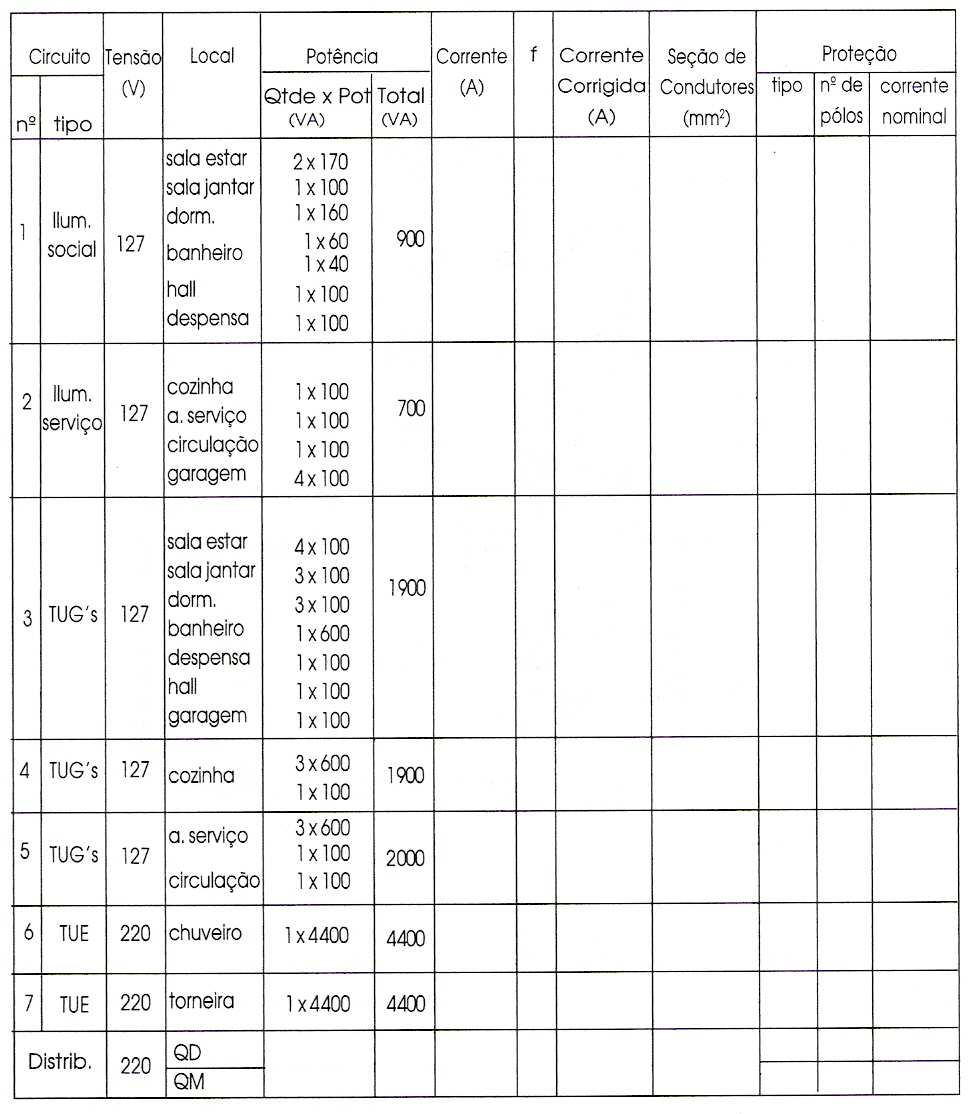
\includegraphics[width=0.55\linewidth]{Figuras/Ch05/fig16}
\end{frame}


\begin{frame}{Divisão da instalação em circuitos terminais}
	\begin{block}{Tensão dos circuitos}
		De acordo com o número de fases e a tensão secundária de fornecimento, devemos observar as seguintes \textbf{recomendações} quanto à determinação da \textbf{tensão de ligação} dos circuitos terminais:
		\begin{itemize}
			\item Quando a instalação for \textbf{monofásica}, todos os circuitos terminais terão ligação \textbf{fase-neutro}, na tensão de fornecimento padronizada da concessionária local;
			\item Quando a instalação tiver \textbf{duas ou três fases}, deve-se ter os circuitos de iluminação e tomadas de uso geral no \textbf{menor valor de tensão}, isto é, estes circuitos serão \textbf{monofásicos} (ligação fase-neutro);
		\end{itemize}
	\end{block}
\end{frame}


\begin{frame}{Divisão da instalação em circuitos terminais}
	\begin{block}{Tensão dos circuitos}
		\begin{itemize}
			\item Quando a instalação tiver \textbf{duas ou três fases}, e a \textbf{maior das tensões} (fase-fase) for \textbf{até \SI{230}{\volt}}, pode-se ter circuitos de tomadas de uso específico ligados em duas fases (circuitos bifásicos) ou circuitos entre uma fase e o neutro (circuitos monofásicos).
			\item Nestes casos, geralmente utilizam-se circuitos \textbf{bifásicos} (\SI{220}{\volt}, por exemplo) para os aparelhos de \textbf{uso específico} de maior potência, tais como chuveiros elétricos, torneiras elétricas e aparelhos de ar-condicionado.
		\end{itemize}
	\end{block}
\end{frame}


\begin{frame}{Divisão da instalação em circuitos terminais}
	\begin{block}{}
		A figura abaixo mostra a divisão de uma instalação elétrica residencial em diversos circuitos terminais.
	\end{block}

	\centering
	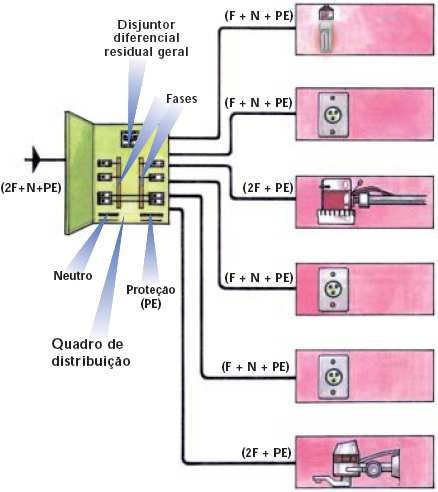
\includegraphics[width=0.45\linewidth]{Figuras/Ch05/fig17}
\end{frame}


\section*{Exercícios}
\frame{
	\frametitle{Exercícios}
	\begin{block}{}
		01. Como você faria a divisão de circuitos da sua casa? Esboce uma tabela.
	\end{block}
}

\section*{Referências}

\frame{
	\frametitle{Referências e Exercícios Complementares}
	\begin{itemize}
		\item CREDER, Hélio; Instalações Elétricas, 14ª edição, Editora LTC, Rio de Janeiro, 2004.
		\item Manual de Instalações Elétricas - Prysmian.
	\end{itemize}
	%\centering{\alert{Página 36 - \textbf{1.6.1 até 1.6.5, 1.6.17 até 1.6.19}}} \\
	%	\centering{\alert{Lista de exercícios 01}}
}